
%Не забыть:
%--------------------------------------
%Вставить колонтитулы, поменять название на титульнике



%--------------------------------------

\documentclass[a4paper, 12pt]{article} 

%--------------------------------------
%Russian-specific packages
%--------------------------------------
%\usepackage[warn]{mathtext}
\usepackage[T2A]{fontenc}
\usepackage[utf8]{inputenc}
\usepackage[english,russian]{babel}
\usepackage[intlimits]{amsmath}
\usepackage{esint}
%--------------------------------------
%Hyphenation rules
%--------------------------------------
\usepackage{hyphenat}
\hyphenation{ма-те-ма-ти-ка вос-ста-нав-ли-вать}
%--------------------------------------
%Packages
%--------------------------------------
\usepackage{amsmath}
\usepackage{amssymb}
\usepackage{amsfonts}
\usepackage{amsthm}
\usepackage{latexsym}
\usepackage{mathtools}
\usepackage{epstopdf}
\usepackage{etoolbox}%Булевые операторы
\usepackage{extsizes}%Выставление произвольного шрифта в \documentclass
\usepackage{geometry}%Разметка листа
\usepackage{indentfirst}
\usepackage{wrapfig}%Создание обтекаемых текстом объектов
\usepackage{fancyhdr}%Создание колонтитулов
\usepackage{setspace}%Настройка интерлиньяжа
\usepackage{lastpage}%Вывод номера последней страницы в документе, \lastpage
\usepackage{soul}%Изменение параметров начертания
\usepackage{hyperref}%Две строчки с настройкой гиперссылок внутри получаеммого
\usepackage[usenames,dvipsnames,svgnames,table,rgb]{xcolor}% pdf-документа
\usepackage{multicol}%Позволяет писать текст в несколько колонок
\usepackage{cite}%Работа с библиографией
\usepackage{subfigure}% Человеческая вставка нескольких картинок
\usepackage{tikz}%Рисование рисунков
\usepackage{float}
% Для картинок Моти
\usepackage{misccorr}
\usepackage{lscape}
\usepackage{cmap}


\usepackage{graphicx,xcolor}
\graphicspath{{Pictures/}}
\DeclareGraphicsExtensions{.pdf,.png,.jpg}

%----------------------------------------
%Список окружений
%----------------------------------------
\newenvironment {theor}[2]
{\smallskip \par \textbf{#1.} \textit{#2}  \par $\blacktriangleleft$}
{\flushright{$\blacktriangleright$} \medskip \par} %лемма/теорема с доказательством
\newenvironment {proofn}
{\par $\blacktriangleleft$}
{$\blacktriangleright$ \par} %доказательство
%----------------------------------------
%Список команд
%----------------------------------------



\newcommand{\grad}
{\mathop{\mathrm{grad}}\nolimits} %градиент

\newcommand{\diver}
{\mathop{\mathrm{div}}\nolimits} %дивергенция

\newcommand{\Def}[1]
{\underline{\textbf{#1}}} %определение

\newcommand{\RN}[1]
{\MakeUppercase{\romannumeral #1}} %римские цифры

\newcommand {\theornp}[2]
{\textbf{#1.} \textit{ #2} \par} %Написание леммы/теоремы без доказательства

\newcommand{\qrq}
{\ensuremath{\quad \Rightarrow \quad}} %Человеческий знак следствия

\newcommand{\qlrq}
{\ensuremath{\quad \Leftrightarrow \quad}} %Человеческий знак равносильности

\renewcommand{\phi}{\varphi} %Нормальный знак фи

\newcommand{\me}
{\ensuremath{\mathbb{E}}}

\newcommand{\md}
{\ensuremath{\mathbb{D}}}



%\renewcommand{\vec}{\overline}




%----------------------------------------
%Разметка листа
%----------------------------------------
\geometry{top = 3cm}
\geometry{bottom = 2cm}
\geometry{left = 0.7cm}
\geometry{right = 0.7cm}
%----------------------------------------
%Колонтитулы
%----------------------------------------
\pagestyle{fancy}%Создание колонтитулов
\fancyhead{}
%\fancyfoot{}
\fancyhead[C]{\textsc{Поляризация}}%Вставить колонтитул сюда
%----------------------------------------
%Интерлиньяж (расстояния между строчками)
%----------------------------------------
%\onehalfspacing -- интерлиньяж 1.5
%\doublespacing -- интерлиньяж 2
%----------------------------------------
%Настройка гиперссылок
%----------------------------------------
\hypersetup{				% Гиперссылки
	unicode=true,           % русские буквы в раздела PDF
	pdftitle={Заголовок},   % Заголовок
	pdfauthor={Автор},      % Автор
	pdfsubject={Тема},      % Тема
	pdfcreator={Создатель}, % Создатель
	pdfproducer={Производитель}, % Производитель
	pdfkeywords={keyword1} {key2} {key3}, % Ключевые слова
	colorlinks=true,       	% false: ссылки в рамках; true: цветные ссылки
	linkcolor=blue,          % внутренние ссылки
	citecolor=blue,        % на библиографию
	filecolor=magenta,      % на файлы
	urlcolor=cyan           % на URL
}
%----------------------------------------
%Работа с библиографией (как бич)
%----------------------------------------
\renewcommand{\refname}{Список литературы}%Изменение названия списка литературы для article
%\renewcommand{\bibname}{Список литературы}%Изменение названия списка литературы для book и report
%----------------------------------------
\begin{document}
\begin{titlepage}
\begin{center}
\textsc{Национальный исследовательский университет "Высшая школа экономики"\\[5mm]
Факультет Физики}

\vfill

\textbf{ОТЧЁТ ПО ЛАБОРАТОРНОЙ РАБОТЕ \\[3mm]
"ПОЛЯРИЗАЦИЯ"\\[3mm]
по курсу "Оптика"
\\[20mm]
}
\end{center}

\hfill
\begin{minipage}{.5\textwidth}
Выполнила:\\[2mm] 
Фазлиахметова Олеся Камилевна\\
БФЗ193\\
2 курс\\[5mm]

Проверила:\\[2mm] 
Готовко С. К. 
\end{minipage}%
\vfill
\begin{center}
 Москва\\
 \today
\end{center}
\end{titlepage}



\tableofcontents

\newpage

	\section{Цель работы}

Перед началом выполнения работы были поставлены следующие цели:

\begin{enumerate}
	
	\item Поляризация

\begin{enumerate}


	\item Определить поляризацию света от источника.

	\item Проверить справедливость закона Малюса.

	\item Определить главные направления пластинок $\lambda$/2 и  $\lambda$/4 по отношению к входному поляризатору.

	\item Определить степень поляризации света после прохождения пластинок $\lambda$/2 и  $\lambda$/4, одна из осей которых повернута под углом 45º по отношению ко входному поляризатору. Для линейно поляризованного света определить также направление поляризации по отношению к разрешенному направлению входного поляризатора. Повторить для нескольких углов поворота пластинок.

	\item Определить тип ($\lambda$/2 или $\lambda$/4) для неизвестной пластинки.

\end{enumerate}

	\item Угол Брюстера и формулы Френеля

\begin{enumerate}

	\item С помощью черного зеркала (зеркала Ллойда) или стеклянной пластины определить положение разрешенного направления в поляризаторе.

	\item Определить величину угла Брюстера для черного зеркала или стеклянной пластинки и коэффициент преломления.

	\item Измерить интенсивность отраженного излучения для черного зеркала или стеклянной пластинки для различных углов падения и двух поляризаций (s и p). Проверить справедливость формул Френеля. 

\end{enumerate}
\end{enumerate}

\section{Оборудование}

\begin{enumerate}

	\item Лазер;

	\item Поляризатор;

	\item Пластинки  ($\lambda$/2 и $\lambda$/4);

	\item Подставки и крепления для элементов оптической схемы;

	\item Линейки.

	\item Черное зеркало

\end{enumerate}

\section{Теоретическое описание}


\subsection{Поляризация}
Свет — это электромагнитная волна. Такие волны - поперечные, в них направления векторов E и H взаимно перпендикулярны и располагаются в плоскости, перпендикулярной направлению распространения волны. При этом положение векторов E и H в световой волне в пространстве может различным образом меняться со временем. Характер этого изменения говорит о поляризации света. Далее, для простоты будем следить только за вектором электрического поля E.


В простейшем случае направление вектора E в пространстве может меняться со временем случайным образом. Это справедливо для большинства обычных источников света, в которых излучение создается большим количеством некогерентно испускающих свет атомов. В таком случае говорят об \textbf{естественном или неполяризованном свете}.


Возможен также случай, когда ориентация вектора E не меняется со временем. Такой свет называется \textbf{линейно поляризованным} или, иначе, плоско поляризованным. В линейно поляризованной волне плоскость, в которой находятся вектор E и вектор направления распространения волны, называется плоскостью колебаний.


Колебания электрического поля в плоско поляризованной волне можно разложить на две взаимно перпендикулярных компоненты. В этом случае сдвиг фаз между колебаниями каждой из компонент равен нулю (или целому кратному $\pi$). Однако, в самом общем случае, сдвиг фаз между ними может быть произвольным, тогда вектор E со временем будет описывать эллипс в пространстве. В этом случае говорят об эллиптически поляризованном свете. Если разность фаз колебаний составляет $\pi$/2 (или кратен $\pi$/2), вектор E описывает окружность и в этом случае говорят о \textbf{круговой поляризации света}. 




Важно отметить отличие между эллиптически поляризованного и неполяризованного света. Несмотря на то, что в обоих случаях наблюдаются колебания электрического поля в любых взаимно перпендикулярных направлениях, в первом случае эти колебания происходят согласованно, с фиксированной разностью фаз. Во втором же случае эти колебания не согласованы.



Плоско-поляризованный свет обычно получают с помощью специальных устройств — поляризаторов. После прохождения естественного света через поляризатор, получается линейно поляризованный свет. Направление колебаний электрического вектора в полученном линейно поляризованном свете называется \textbf{разрешенным направлением поляризатора}. Также поляризатор можно использовать не только для получения света определенной поляризации, но и для определения его поляризации. В этом случае поляризатор могут называть анализатором.

\subsection{Получение плоско-поляризованного света}

Существует несколько способов получения плоско-поляризованного света.


На практике часто используются поляризаторы, чей принцип действия основан на явлении дихроизма, состоящее в различном поглощении света веществом в зависимости от поляризации. У некоторых кристаллов (например, у турмалина) различие коэффициента поглощения для света с перпендикулярными направлениями поляризации может быть настолько сильным, что даже при небольшой толщине кристалла при прохождении поглощается полностью одна из компонент. В итоге, на выходе получается линейно поляризованный свет.



Рассмотрим пластинку, изготовленную из материала, обладающего свойством двулучепреломления, стороны которой параллельной оптической оси материала. Из-за различия коэффициентов преломления свет с поляризацией вдоль оси и перпендикулярной ей проходит сквозь пластинку за разное время. Поэтому после прохождения пластинки появится разность фаз между по-разному поляризованными волнами. Если разность фаз после прохождения пластинки меняется на $\pi$/2, то ее называют четвертьволновой пластинкой или пластинкой $\lambda$/4. Если же изменение составляет $\pi$, то это полуволновая пластинка или пластинка $\lambda$/2. Важно отметить, что подобное справедливо только для определенной длины волны падающего света. Для других длин волн разность фаз будет отличаться: для больших длин волн разность фаз будет меньше, и наоборот, для меньших длин волн разность фаз будет больше.








\section{Выполнение работы}

\subsection{Определение поляризации света от источника.}

Если свет является суммой неполяризованного и линейно поляризованного, то его можно охарактеризовать степенью поляризации P, которой называется величина:

\begin{equation}
P = \frac{I_{max}-I_{min}} {I_{max}+I_{min}} 
\end{equation}

где $I_{max}$ и  $I_{min}$ – максимальная и минимальная интенсивности частично поляризованного света, пропускаемого анализатором. Для естественного света она равна 0, для плоско
поляризованного 1. Эллиптически поляризованный свет этой величиной характеризовать не принято.


 Значения $I_{min}$ и $I_{max}$ для нашего лазера: $I_{min} = 73\pm 0.4 $ мкВт,    $I_{max} = 638 \pm 3$ мкВт. Тогда $P = 0.79\pm 0.01$. Вывод: наш свет не является ествественным  или плоско-поляризованным, он смешанный.








\subsection{Проверка справедливости закона Малюса.}

Интенсивность линейно поляризованного света $I_0$, после прохождения через анализатор, разрешенное направление которого составляет угол $\alpha$ к плоскости колебаний, задается законом Малюса:

\begin{equation}
I = I_0 \cos^2\alpha 
\end{equation}


\begin{figure}[H]
	\centering
	\includegraphics[scale=0.7]{Malus}
	\caption{Закон Малюса.}
\end{figure}


\subsection{Определение главных направлений пластинки по отношению к входному поляризатору}
\subsubsection{Пластинка $\lambda/2$:}
Направление максимума:


\begin{center}
\begin{tabular}{ c c }

Угол, $^o$ & Мощность, мкВт\\
$195\pm 5$ &$476\pm2$\\
$285\pm 5 $& $476\pm2$\\
\end{tabular}
\end{center}
Направление минимума:

\begin{center}
\begin{tabular}{ c c }

Угол, $^o$ & Мощность, мкВт\\
$330\pm 5 $&$8.8\pm0.01$\\
$60 \pm 5$& $6.6\pm0.01$\\
\end{tabular}
\end{center}


\subsubsection{Пластинка $\lambda/4$:}

Четвертьволновая пластина создает фазовый сдвиг величиной в четверть длины волны. Если входной пучок линейно поляризован, и плоскость поляризации расположена под углом 45$^o$ к быстрой или медленной оси волновой пластины, то выходное излучение будет поляризовано циркулярно.

Направление максимума:


\begin{center}
\begin{tabular}{ c c }

Угол, $^o$ & Мощность, мкВт\\
$260\pm 5$ &$533\pm3$\\
$350\pm 5$ & $530\pm2$\\
\end{tabular}
\end{center}
Направление минимума (круговая поляризация):

\begin{center}
\begin{tabular}{ c c }

Угол, $^o$ & Мощность, мкВт\\
$305\pm 5 $&$380\pm2$\\
$215\pm 5 $& $354\pm2$\\
\end{tabular}
\end{center}


		\subsection{Опеределение степени поляризации после прохождения пластинок}


	\subsubsection{Пластинка $\lambda/2$:}
Для линейно поляризованного света определим направление поляризации по отношению к разрешенному направлению входного поляризатора:
\begin{center}
\begin{tabular}{ |c |c |}
\hline
Угол пластинки, $^o$  &Угол анализатора, $^o$\\
\hline
$15\pm 5 $ &$30 \pm 5 $ \\
$30\pm 5$ &$60\pm 5 $ \\
$45\pm 5$ & $90\pm 5 $  \\
\hline
\end{tabular}
\end{center}
Вывод: угол поляризации после прохождения пластинки  в два раза больше угла поляризации после прохождения поляризатора.

Определим степень поляризации света после прохождения пластинки, ось которой повернута под углом 45º по отношению ко входному поляризатору:
\begin{center}
\begin{tabular}{ c c }
$I_{max} $ &$466\pm3$ мкВт\\
$I_{min}$ & $6\pm0.01$ мкВт\\
\end{tabular}
\end{center}

\[P =0.97 \]

	\subsubsection{Пластинка $\lambda/4$:}
Для линейно поляризованного света определим направление поляризации по отношению к разрешенному направлению входного поляризатора:
\begin{center}
\begin{tabular}{ |c |c |}
\hline
Угол пластинки, $^o$  &Угол анализатора, $^o$\\
\hline
$90\pm 5 $ &180 \\
$90\pm 5$ &360 \\
$180\pm 5$ & 0 \\
\hline
\end{tabular}
\end{center}

Определим степень поляризации света после прохождения пластинки, ось которой повернута под углом 45º по отношению ко входному поляризатору:

\begin{center}
\begin{tabular}{ c c }
$I_{max} $ &$301\pm2$ мкВт\\
$I_{min}$ & $195\pm1$ мкВт\\
\end{tabular}
\end{center}

\[P =0.21 \pm0.01 \]



		\subsection{Опеределение типа пластинок}

			\subsubsection{Пластинка №1}
\begin{center}
\begin{tabular}{ c c }
Угол пластинки, $^o$ & Интенсивность, мкВт\\
$325\pm 5 $&$470\pm3$\\
$10\pm 5 $& $281\pm1$\\
$55\pm 5$ & $537\pm3$\\
\end{tabular}
\end{center}


			\subsubsection{Пластинка №2}
\begin{center}
\begin{tabular}{ c c }
Угол пластинки, $^o$ & Интенсивность, мкВт\\
$350\pm 5 $&$510\pm3$\\
$35\pm 5 $& $325\pm2$\\
$80\pm 5$ &$498\pm3$\\
\end{tabular}
\end{center}

Обе пластинки  $\lambda/4$


		\subsection{Опеределение положения разрешенного направления в поляризаторе и угла Брюстера}

Определить направление разрешенных колебаний поляроида проще всего с помощью черного зеркала. При падении света на отражающую поверхность под углом Брюстера свет в отраженном луче полностью поляризован, а вектор \textbf{E} параллелен отражающей поверхности (p-поляризация). Луч света, прошедщий поляроид и отразившийся от черного зеркала, имеет минимальную интенсивность при выполнении двух условий: во-первых, свет падает на отражающую поверхность под углом Брюстера, во-вторых, в падающем пучке вектор \textbf{E} лежит в плоскости падения. Вращая поляроид вокруг направления луча и черное зеркало вокруг направления оси, перпендикулярной лучу, находим минимальную яркость луча, отраженного от зеркала, и таким образом определяем разрешенное направление поляроида и угол Брюстера.\\

Соответственно, величина угла Брюстера связана с показателем преломления материала:
\begin{equation}
\tg \theta_i=n
\end{equation}

\textbf{Положение определенного направления в поляризаторе:}
\[\alpha = 260\pm 5^o\]

\textbf{Угол Брюстера}
\[\theta = 52\pm1^o\]

\[n = \tg 52\pm 1^o= 1.28\pm 0.05\]

		\subsection{Проверка справедливости формул Френеля}
В общем случае, прохождение и отражение света описывается формулами Френеля. Согласно этим соотношениям, коэффициент отражения зависит от поляризации падающей электромагнитной волны. Принято выделять s-поляризацию, когда вектор электрического поля перпендикулярен плоскости падения, и p-поляризацию, когда вектор электрического поля лежит в плоскости падения. 

\begin{figure}[H]
	\centering
	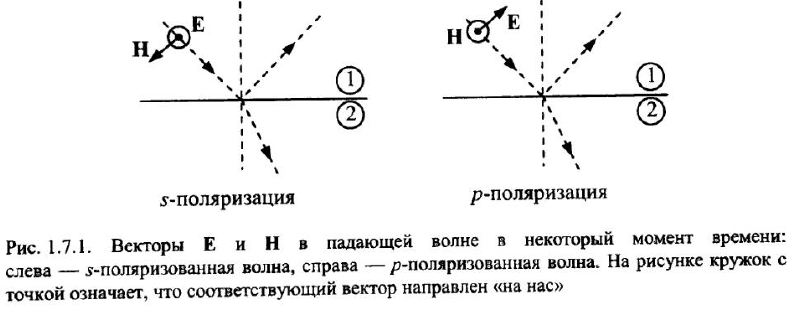
\includegraphics[scale=0.7]{polar}
	\caption{}
\end{figure}


Тогда, для случая падения электромагнитной волны из среды с показателем преломления $n_1$ на плоскую границу со средой с показателем преломления $n_2$ коэффициенты отражения равны:
\begin{equation}
R_s = \left| \frac{n_1\cos\alpha-n_2\cos\gamma}{n_1\cos\alpha+n_2\cos\gamma} \right|^2
\end{equation}
\begin{equation}
R_p = \left| \frac{n_1\cos\gamma-n_2\cos\alpha}{n_1\cos\gamma+n_2\cos\alpha} \right|^2
\end{equation}
где $\alpha$, $\gamma$ – соответственно угол падения и угол прохождения.

Среднеквадратичное отклонение: 
\[\sigma_s = 0.06\]
\[\sigma_p = 0.03\]
\begin{figure}[H]
	\centering
	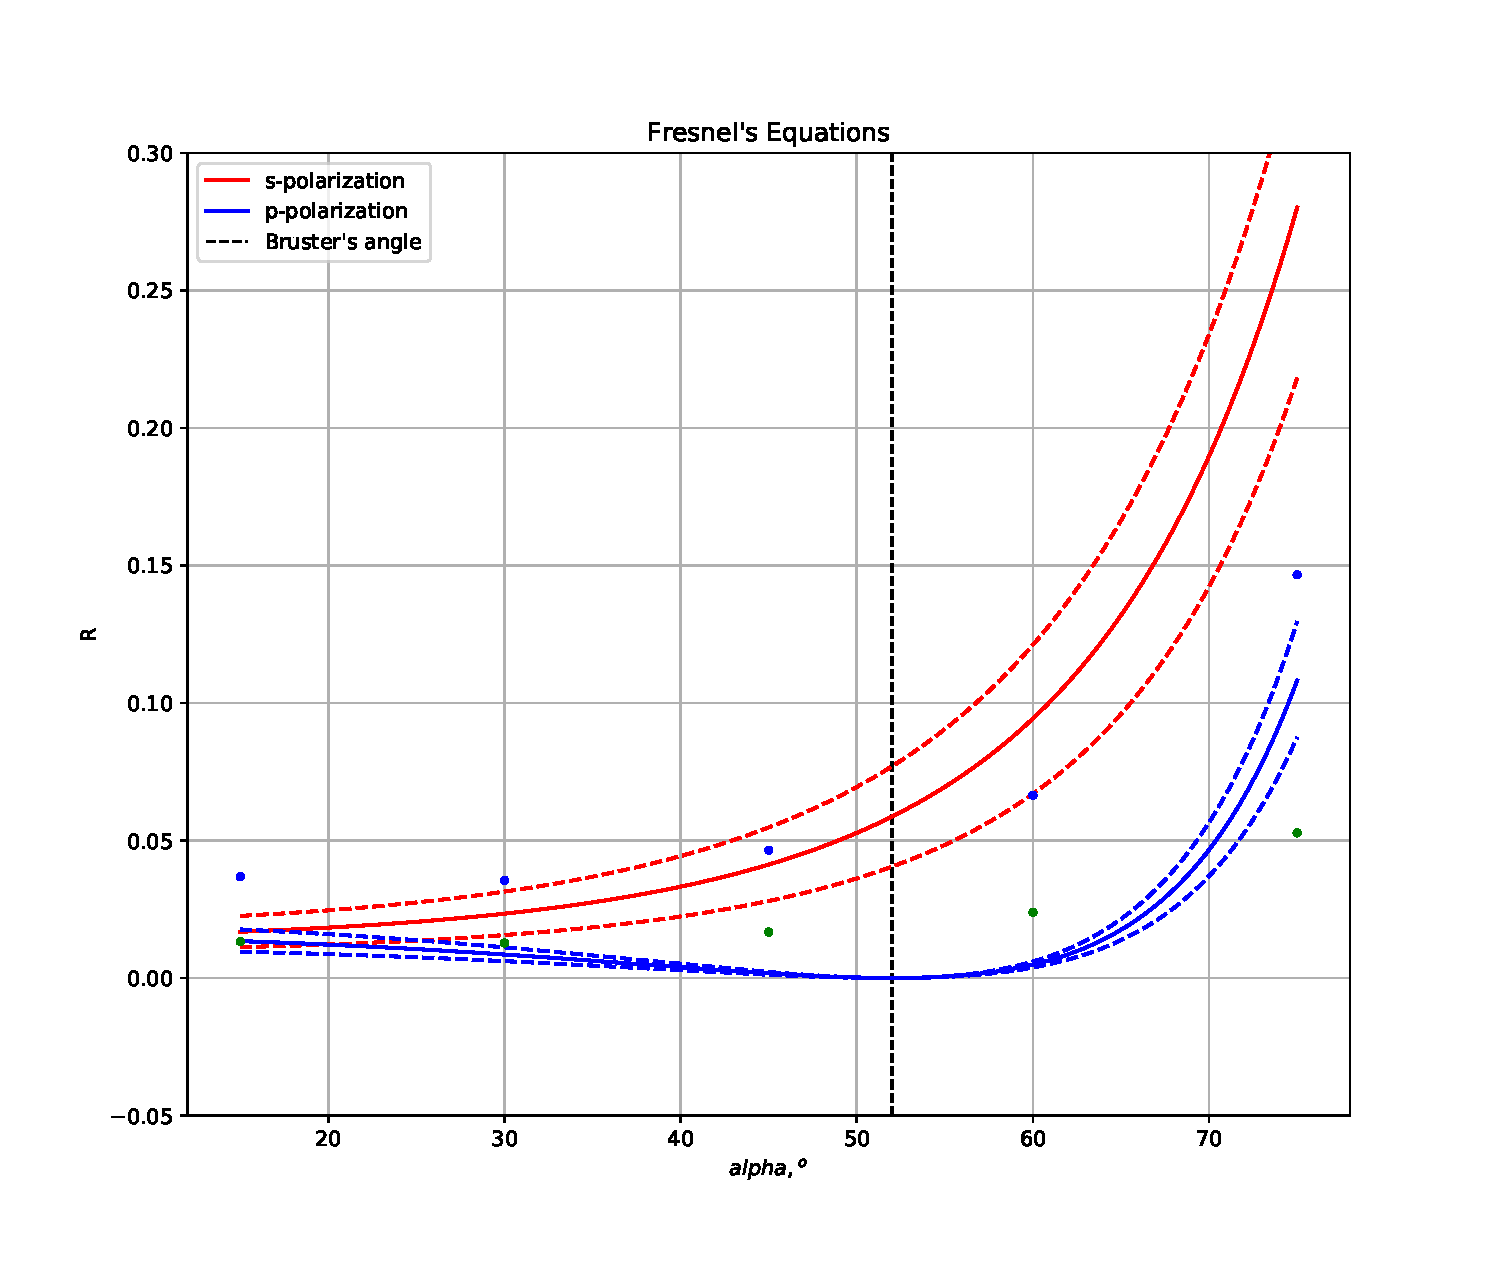
\includegraphics[scale=0.7]{frenel}
	\caption{Уравнения Френеля}
\end{figure}


\section{Вывод}

В ходе работы мы
\begin{enumerate}

	
	\item Поляризация

\begin{enumerate}


	\item Определили поляризацию света от источника.

	\item Проверили справедливость закона Малюса.

	\item Определили главные направления пластинок $\lambda$/2 и  $\lambda$/4 по отношению к входному поляризатору.

	\item Определили степень поляризации света после прохождения пластинок $\lambda$/2 и  $\lambda$/4, одна из осей которых повернута под углом 45º по отношению ко входному поляризатору. Для линейно поляризованного света определили также направление поляризации по отношению к разрешенному направлению входного поляризатора. Повторили для нескольких углов поворота пластинок.

	\item Определили тип ($\lambda$/2 или $\lambda$/4) для неизвестной пластинки.

\end{enumerate}

	\item Угол Брюстера и формулы Френеля

\begin{enumerate}

	\item С помощью черного зеркала (зеркала Ллойда) определили положение разрешенного направления в поляризаторе.

	\item Определили величину угла Брюстера для черного зеркала и коэффициент преломления.

	\item Измерили интенсивность отраженного излучения для черного зеркала для различных углов падения и двух поляризаций (s и p). Проверили справедливость формул Френеля. 

\end{enumerate}
\end{enumerate}
\end{document}